\documentclass{article}

\usepackage{graphicx}
\usepackage[hidelinks]{hyperref}
\usepackage[a4paper, total={6in, 8in}]{geometry}
\usepackage[slovak]{babel}
\usepackage{caption}
\usepackage{subcaption}
\usepackage{listings}

\graphicspath{./include/}

\renewcommand{\figurename}{Obr.}
\renewcommand{\contentsname}{Obsah}

\begin{document}

\begin{titlepage}
	\null\vfill

	\begin{center}
		{\Huge Magnetická levitácia }
		\vskip 2cm

		{\Large Cvičenie č. 8}
		\vskip 0.5cm

		{\large Spojité procesy}
	\end{center}

	\vfill
	\vfill

	\begin{flushright}
		Filip Lobpreis \\
		Matúš Machata \\
		\small\today\\
	\end{flushright}
	\hfill
\end{titlepage}

\thispagestyle{empty}
\clearpage

\tableofcontents
\thispagestyle{empty}
\clearpage

\section{Zadanie}
\label{sec:zadanie}

\begin{figure}[!htbp]
	\begin{center}
		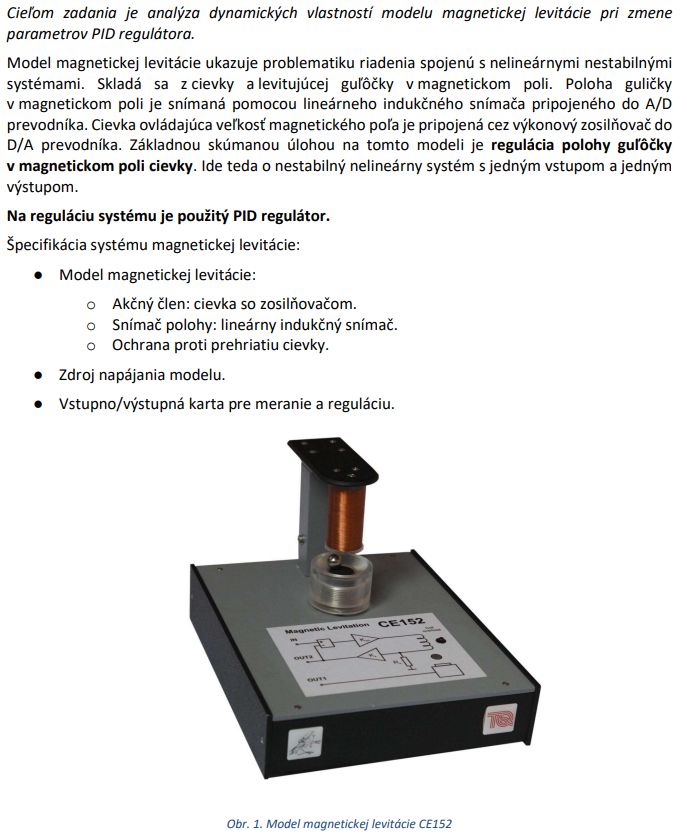
\includegraphics[width=0.95\textwidth]{include/zadanie.png}
	\end{center}
	\caption{Zadanie č. 8 z~predmetu Spojité procesy.}
	\label{fig:zadanie}
\end{figure}

\pagenumbering{arabic}
\clearpage

\section{Merania}
\label{sec:merania}

Ôsme zadanie z~predmetu spojité procesy sa zaoberá skúmaním vplyvu zmien koeficientov PID regulátora
na~ovládanie magnetickej levitácia. V~tomto zadaní budeme postupne meniť PID regulátor a~jeho \textbf{Proporcionálnu},
\textbf{Integračnú} a~Derivačnú zložku. Na~obrázku Obr.~\ref{fig:schema} vidíme model magnetickej levitácia,
ktorý sme použili pri~meraniach. Jednotlive parametre regulatora budeme menit v rozsahu $\pm20\%$.

\begin{figure}[!htbp]
	\begin{center}
		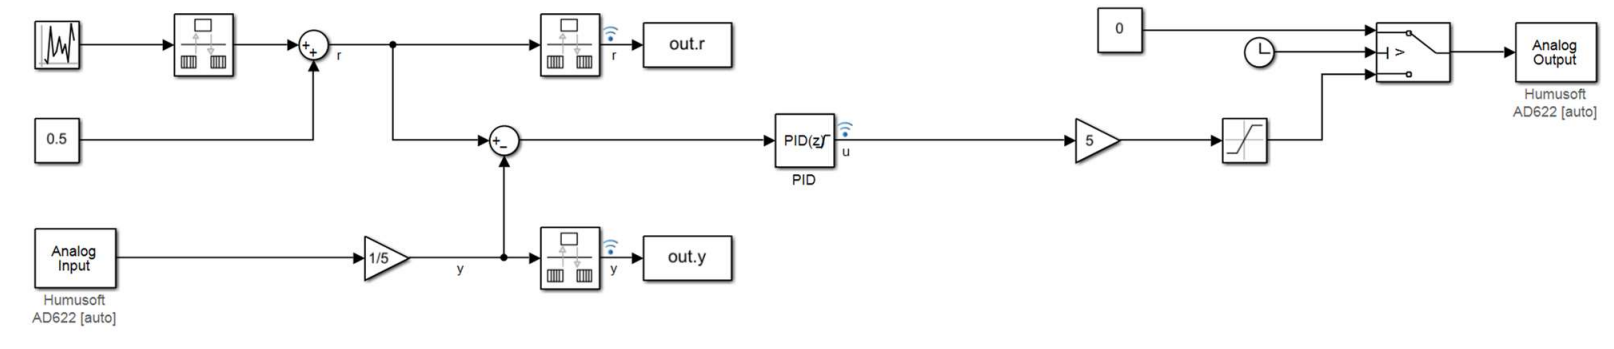
\includegraphics[width=0.95\textwidth]{include/schema.png}
	\end{center}
	\caption{Schéma pre~model magnetickej levitácie.}
	\label{fig:schema}
\end{figure}

\subsection{Meranie 1}
\label{sec:meranie1}



\subsection{Meranie 2}
\label{sec:meranie2}

\subsection{Meranie 3}
\label{sec:meranie3}

\subsection{Meranie 4}
\label{sec:meranie4}

\subsection{Meranie 5}
\label{sec:meranie5}

\subsection{Meranie 6}
\label{sec:meranie6}


\end{document}

